%% ------------------------------------------------------------------------- %%
\chapter{Avaliação}
\label{cap:avaliacao}

Neste capítulo, apresentamos experimentos realizados com o Enactment Engine com objetivo de avaliar
seu uso, contrastando com soluções \emph{ad-hoc} de implantação automatizada.
Também avaliamos seu desempenho e escalabilidade para verificar a viabilidade de seu uso
no contexto de composições de serviços de grande escala.

\section{Implantando coreografias com e sem o EE}
\label{sec:avaliacao_eng_sw}

Nesta seção, nós avaliamos como o \ee melhora o processo de implantação
pelo fato de ser uma solução baseada em middleware.
Para essa avaliação, desenvolvemos uma solução \emph{ad-hoc}
para a implantação de uma coreografia particular.
A ``coreografia do aeroporto'' é um exemplo fornecido por especialistas
no domínio aeroportuário~\cite{Choreos2012D6.2} e que contém 15 serviços.
Também implantamos a mesma coreografia utilizando o EE.
Ambas as soluções estão disponíveis em \url{https://github.com/choreos/airport_enactment}.

Para implantar a coreografia do aeroporto com o EE, escrevemos
a especificação da coreografia e o programa cliente para invocar o EE,
disparando assim a implantação.
A especificação da coreografia foi escrita com objetos Java em 40 minutos,
contendo 162 linhas de código (LoC), uma média de 11 linhas por serviço.
O autor dessa especificação foi um aluno de doutorado, já acostumado ao conceito
de coreografias de serviços web, e que contribuiu com o código do EE.
O programa cliente, a classe \texttt{AirportEnact}, utiliza a API Java do EE,
tem apenas 22 linhas de código, e foi escrito pelo autor desta dissertação
em menos de 5 minutos.
Depois que essas classes foram escritas, a implantação da coreografia em
três nós, utilizando o EE, levou apenas 4 minutos.

Para desenvolver a solução \emph{ad-hoc} foi necessário aproximadamente
9 horas de desenvolvimento de um programador (o autor desta dissertação), e mais 60 minutos
para o mesmo programador executar a implantação, distribuindo os 15
serviços por três nós alvos.
Essa solução precisou da escrita de 
100 LoC de shell scripts, 220 LoC de Java, and 85 LoC de Ruby (para o Chef). 

No restante desta seção, descreveremos o processo de criação e execução
da solução \emph{ad-hoc}. Destacaremos as dificuldades no processo
que o implantador encontra sem o uso do EE.

\paragraph{Implementação da solução ad hoc}
A implantação de cada serviço é executada por uma receita Chef contida em um \emph{cookbook}.
Nós escrevemos um \emph{cookbook} modelo, para implantar pacotes JARs,
e o usamos para gerar \emph{cookbooks} para os 15 serviços participantes.
O processo de criar os 15 \emph{cookbooks} foi parcialmente automatizado
pelo \script \texttt{generate} que escrevemos.
As URLs dos pacotes dos serviços tiveram que ser manualmente inseridas nos
\emph{cookbooks} depois da execução da \script \texttt{generate}.

Para implementar o enlace entre serviços,
desenvolvemos um pequeno mas não trivial programa Java, chamado \texttt{context\_sender}. 
Ele é responsável por invocar a operação \texttt{setInvocationAddress} de um dado serviço.
Implementamos o \texttt{context\_sender} como um programa Java para
aproveitar a API SOAP fornecida pelo ambiente Java SE.
Também desenvolvemos o \script \texttt{bind\_services},
responsável por executar o programa \texttt{context\_sender}
para cada dependência presente na coreografia.
Uma vez que os IPs dos serviços são conhecidos apenas após a implantação,
o \script \texttt{bind\_services} é na verdade um modelo com lacunas
que devem ser manualmente preenchidas com os IPs dos serviços implantados.

A execução da solução \emph{ad-hoc} possui vários passos,
inclusive alguns manuais.
Para cada nó alvo, o implantador deve se conectar ao nó (via SSH),
instalar o git, baixar os \emph{cookbooks}, executar o \script \texttt{install\_chef} 
para instalar o Chef, editar alguns arquivos de configuração para definir
quais serviços serão implantados no nó, e executar o Chef-Solo.
Após implantar os serviços, o implantador deve editar o \script
\texttt{bind\_services} com os IPs dos serviços implantados
e, finalmente, executar o \script \texttt{bind\_services}.
Alguns dos problemas dessa solução \emph{ad-hoc} são:

\begin{itemize}

\item Três diferentes tecnologias são utilizadas:
shell script, Java e Chef.
Conhecimento de linha de comando também foi necessária em alguns passos,
como utilizar o editor \emph{vim} ou o comando \texttt{ps} para verificar
o estado dos processos dos serviços implantados.
Isso sugere que se requer uma ampla gama de habilidades técnicas
do desenvolvedor de soluções de implantação.
Algumas dessas habilidades, como utilizar o Chef,
são notoriamente não-fáceis de se aprender.
O código Java utilizado para realizar a invocação de serviços SOAP
pode também ser considerado como não-trivial para um programador
não acostumado com o padrão SOAP.

\item Replicação de código nos \emph{cookbooks} gerados.
Se algo muda no modelo, é preciso regenerar todos os \emph{cookbooks}
e realizar a edição manual também.
Contudo, as edição manuais mencionadas
poderiam ser evitadas com um \script mais complexo.
Replicação de código poderia também ter sido evitada com a criação de um
``LWRP'' (\emph{light weight resource provider}) do Chef,
mas isso seria uma tarefa para usuários avançados do Chef.

\item Para cada nó alvo, o implantador deve realizar alguns passos manuais
que são demorados. Alguns deles (executar \texttt{install\_chef}, por exemplo)
poderiam ser evitados com a utilização de uma ferramenta como
Capistrano\footnote{\url{http://www.capistranorb.com/}},
mas isso demandaria mais uma tecnologia a ser aprendida.
Outros passos manuais, como a edição de arquivos de configuração, 
são bastante propensos a erros.
Esquecer-se de vírgulas ou digitar errado o nome de serviços
são erros bem prováveis de acontecerem.

\item Há muita pouca paralelização no processo.
Com os \scripts construídos, o implantador poderia melhorar
um pouco o paralelismo utilizando ferramentas como o
Byobu\footnote{\url{http://byobu.co/}} 
para digitar o mesmo comando em várias máquinas.
Mas isso demandaria mais uma habilidade a ser aprendida pelo implantador,
além de ser uma forma muito limitada de escalar o processo.

\end{itemize}

Nesse exemplo, usamos uma composição de apenas 15 serviços.
Composições de grande escala aumentariam muito mais a complexidade da
solução \emph{ad-hoc}.
Para se obter uma solução completa com a abordagem \emph{ad-hoc},
um esforço extra de desenvolvimento seria necessário
para implementar funcionalidades já presentes no EE,
como o tratamento de falhas de terceiros,
atualização de coreografias, seleção dinâmica de nós,
implantação concorrente, etc.
Além disso, para desenvolver a solução \emph{ad-hoc},
utilizamos códigos que já estavam disponíveis no EE,
tais como os modelos dos \emph{cookbooks} e o \texttt{context\_sender}.
Implantadores teriam que começar tudo do zero.

Nós reconhecemos que essa avaliação por comparação com uma solução \emph{ad-hoc}
tem suas limitações, uma vez que os resultados dependem fortemente das
habilidades técnicas do implantador.
Conduzir um experimento rigoroso de engenharia de software com vários
desenvolvedores assumindo o papel de implantador traria uma evidência melhor.
Contudo, acreditamos que a avaliação descrita aqui já é o suficiente
para expandir nosso entendimento sobre o valor agregado por uma solução
com suporte de middleware, como o \ee, uma vez que temos agora uma boa ilustração
do esforço necessário para se implantar composições de serviços.

\section{Análise de desempenho e escalabilidade}

Conduzimos experimentos para avaliar o desempenho e escalabilidade do
Enactment Engine em função de sua capacidade de implantar um número significativo
de composições em uma plataforma de nuvem utilizada no mercado.

Nossos experimentos utilizam uma carga sintética modelada conforme ilustrado na Figure~\ref{fig:eval_composition}.
A direção das flechas vão do serviço consumidor para o provedor.
Embora respostas não sejam representadas por questão de simplicidade,
elas são sempre enviadas sincronamente.
Essa topologia foi escolhida porque 1) é um exemplo representativo de processos de negócios
(potencialmente compostos por ramificações -- chamadas para outros sistemas -- e junções correspondentes)
e 2) segue um padrão repetitivo que pode ser usado para aumentar suavemente o tamanho da composição,
para que possamos analisar o desempenho do EE conforme a carga aumenta.


\begin{figure}[h]
  \centering
  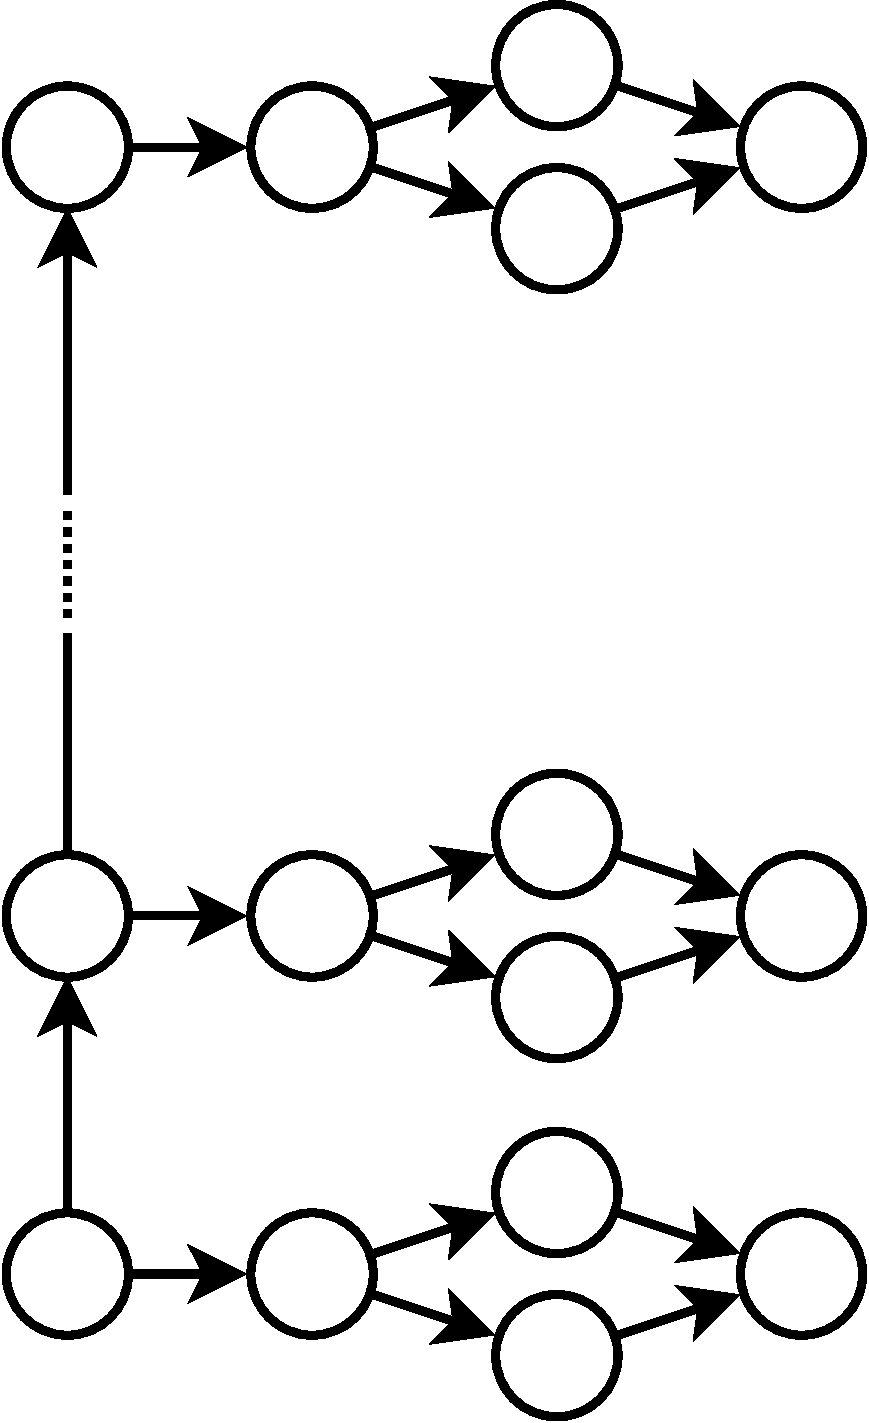
\includegraphics[scale=0.25, angle=270]{eval_composition.pdf}
  \caption{Topologia das composições utilizadas em nossos experimentos.}
  \label{fig:eval_composition}
\end{figure}


Inicialmente, conduzimos experimentos
de desempenho do EE implantando composições nos seguintes cenários:
1) um pequeno conjunto de pequenas composições;
2) um pequeno conjunto de composições maiores;
3) um conjunto maior de pequenas composições;
4) uma razão maior de serviços por nó.
A Tabela~\ref{tab:cases} quantifica cada cenário.

\begin{table}
\centering
\caption{Cenários de implantação para os experimentos de desempenho.}
\label{tab:cases}
\begin{tabular}{r r r r c} \hline
\emph{Cenário} & \emph{Composições} & \emph{Tamanho} & \emph{Nós} & \emph{Serviços/Nós} \\ \hline
1 &  10 &  10 &  9 & 11 ou 12 \\
2 &  10 & 100 & 90 & 11 ou 12 \\
3 & 100 &  10 & 90 & 11 ou 12 \\
4 &  10 &  10 &  5 &       20 \\
\hline \end{tabular}
\end{table}

Em nossos experimentos, a política de alocação de nós foi ``cria nós até um limite, e depois faz rodízio entre eles'',
na qual a quantidade de nós utilizados é configurada antes de cada experimento.
Se a quantidade de nós não é divisível pelo número de nós,
alguns nós hospedarão um serviço a mais que outros nós.
O tamanho da reserva de nós ociosos era 5,
e o \emph{timeout} de criação de nós era 300 segundos.
Utilizamos a Amazon EC2 como provedor de infraestrutura,
com instâncias do tipo \emph{small},
cada uma com 1.7 GiB of RAM, uma vCPU com processamento
equivalente a 1.0--1.2 GHz, e executando Ubuntu GNU/Linux 12.04.
O EE foi executado em uma máquina com 8 GB de RAM,
com processador Intel Core i7 CPU de 2.7 GHz e GNU/Linux kernel 3.6.7.
A versão do EE utilizada nos experimentos e os dados coletados estão disponíveis 
on-line\footnote{\url{http://ccsl.ime.usp.br/enactmentengine}}
para garantir a reprodutibilidades dos resultados.

Cada cenário foi executado 30 vezes e a Tabela~\ref{tab:results}
apresenta, para cada cenário, o tempo necessário para implantar
todas as composições mais o tempo para invocá-las, o que é feito
para certificar que elas foram corretamente implantadas.
Os valores são médias com intervalo de confiança de 95\%.
A tabela também mostra quantas composições e serviços foram corretamente implantados.

\begin{table}
\centering
\caption{Resultados experimentais.}
\label{tab:results}
\begin{tabular}{c r@{ $\pm$ }l r@{ $\pm$ }l r@{ $\pm$ }l} \hline

\emph{Cenário} & \multicolumn{2}{c}{\emph{Tempo}} & \multicolumn{2}{c}{\emph{Composições}}   & \multicolumn{2}{c}{\emph{Serviços}}\\
                 & \multicolumn{2}{c}{(s)}           & \multicolumn{2}{c}{\emph{com sucesso}} & \multicolumn{2}{c}{\emph{com sucesso}}\\
\hline
1 &  467.9 &  34.8 & 10.0 & 0   & 100.0 & 0   (100\%) \\
2 & 1477.1 & 130.0 &  9.3 & 0.3 & 999.3 & 0.4 (99.9\%)\\
3 & 1455.2 & 159.1 & 98.9 & 0.8 & 998.5 & 1.3 (99.9\%)\\
4 &  585.2 &  38.1 & 10.0 & 0.1 & 100.0 & 0.1 (100\%)\\
\hline \end{tabular}
\end{table}

Os resultados mostram que o EE escala relativamente bem em termos de serviços sendo implantados.
Do cenário 1 para os cenários 2 e 3, o número de serviços (\emph{Composições * Tamanho}) 
foi multiplicado por 10 (Tabela~\ref{tab:cases}),
e em ambas as situações o tempo de implantação cresceu aproximadamente apenas 3 vezes
(Tabela~\ref{tab:results}). 
Parte da explicação para esse incremento no tempo de implantação
está na ocorrência de falhas da infraestrutura.
Quanto maior a quantidade de serviços implantados, 
maiores são as chances da ocorrência dessas falhas.
E para cada falha que acontece, uma nova tentativa de execução
da rotina correspondente é necessária 
(ver sobre o \emph{invoker} na Seção~\ref{sec:falhas}).

Indo do cenário 1 para o cenário 4, o número de serviços por nó dobrou
(Tabela~\ref{tab:cases}). Nessa situação, os resultados da Tabela (Tabela~\ref{tab:results}) 
mostram que o tempo de implantação cresceu aproximadamente 25\%. Parte dessa sobrecarga foi causada
pelo incremente no número de receitas Chef que devem ser executadas (sequencialmente) nos nós.

Durante os experimentos, observamos que, graças aos mecanismos de tolerância a falhas do EE,
a quantidade de falhas na implantação foi baixa: todos os serviços foram corretamente implantados em mais
de 75\% das execuções.
Por ``falha'' consideramos que um serviço não foi corretamente implantado.
O cenário 1 não apresentou falhas,
enquanto que no cenário 4 houve apenas uma falha.
No cenário 2, a pior situação, foram 3 falhas dentre 1000 serviços.
No cenário 3, houve uma execução com 20 falhas, mas esse foi um evento excepcional,
uma vez que a segunda pior situação contou com apenas 3 falhas.

\fabio{quantas seriam as falhas se não tivéssemos o mecanismo de tolerância?}

Finalmente, observamos que 80\% das execuções não utilizaram a reserva de nós ociosos.
Quando a reserva foi usada, houve um acesso máximo por execução de 6 nós,
mas na maioria das vezes o acesso foi de apenas 1 nó.
Também observamos que o tempo de implantação não foi significativamente afetado
quando falhas no ambiente de nuvem ocorriam,
uma vez que novos nós eram imediatamente recuperados da reserva.


%%%

Também conduzimos experimentos para avaliar o desempenho e escalabilidade do Enactment Engine
em termos de sua capacidade de implantar grandes composições de serviços.
Esses experimentos foram realizados em 5 cenários, nos quais se variou o tamanho das composições sendo implantadas
e a quantidade de nós disponíveis no ambiente de nuvem, enquanto manteve-se a razão de 20 serviços implantados por nó.
Cada cenário foi executado 10 vezes.

A topologia utilizada na composição foi a mesma de antes (Figura~\ref{fig:eval_composition}).
O EE foi executado em uma máquina virtual (8 GiB de RAM e 4 vCPUs)
hospedada na infraestrutura de nossa Universidade.
Os nós alvos criados pelo EE eram instâncias \emph{small} da Amazon EC2 e o \emph{timeout} de criação dos nós era de 250 segundos.
Os tempos médios de implantação, com intervalo de confiança de 95\%, são mostrados na Tabela~\ref{fig:ee_scalability}.

Sobre as falhas de implantação,
as piores execuções de cada cenário tiveram 1, 1, 2, 2, e 4 serviços não implantados corretamente
dentre, 200, 600, 1000, 1400 e 1800 serviços, respectivamente.

\begin{figure}[h]
  \centering
  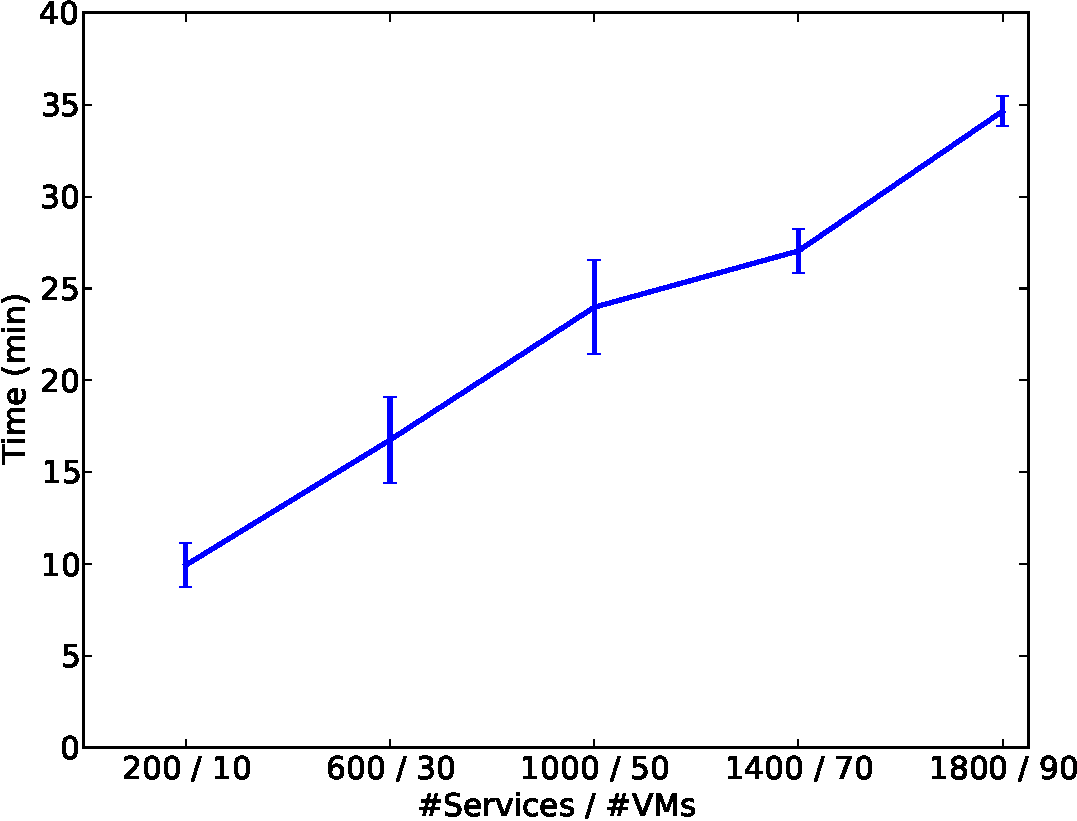
\includegraphics[scale=0.6]{ee_scalability-crop.pdf}
  \caption{Tempos médios de implantação com aumento constante na quantidade de serviços implantados, mantendo-se constante a razão serviços implantados / nós. \todo{traduzir figura}}
  \label{fig:ee_scalability}
\end{figure}

Esses resultados mostram uma boa escalabilidade em termos de serviços implantados.
Aumentando-se 9 em vezes o número de serviços implantados, o tempo de implantação aumentou 3,5 vezes.
Em números absolutos, cada incremento em 400 serviços implantados foi responsável pelo incremento
de 180 a 460 segundos no tempo de implantação.


%\%gerosa{E aquela questão de olhar o real overhead vs o crescimento esperado pela variação estatística do tempo individual de implantação?}
% Questão muito interessante, mas o fato de a distribuição do tempo de implantação
% das coreografias ser quase normal, mas não normal, atrapalha bastante esse tipo de análise. =T

